\documentclass[11pt]{article}
\usepackage[landscape, margin=0.1In]{geometry}
\usepackage{ucs}
\usepackage[utf8x]{inputenc}
\usepackage[T1]{fontenc}
\usepackage[ngerman]{babel}
\usepackage{amsmath,amssymb,amstext}
\usepackage{flowfram}
\usepackage{graphicx}
\usepackage{pgfplots}
\Ncolumn{3}
\usepackage{tabularx}
\setlength{\extrarowheight}{5pt}
\title{Mathe 1 - FHGR Formelsammlung}
\author{André Glatzl}
\date{\today{}, Chur}
\begin{document}
\scriptsize

\noindent
\paragraph{Grundlagen}\mbox{}\\
\paragraph{Symbole}\mbox{}\\
\begin{tabularx}{\columnwidth}{@{}X|X@{}}
    \hline
    $\exists$: Existiert mind. 1 & $\exists!$: Existiert genau 1 \\ \hline
    $\nexists$: Existiert nicht  & $\forall$: Für alle           \\ \hline
\end{tabularx}
\vspace{1mm}

\noindent
\textit{Menge und Elemente gemäss CANTOR}\linebreak
\begin{itemize}
    \item Unter eine Menge verstehen wir jede Zusammenfassung von bestimmten wohlunterschiedenen Objekten (Elemente) unserer Anschauung oder unseres Denkens zu einem Ganzen.
    \item Sei $A$ eine Menge und $x$ ein $Element$ von $A$. Die Aussage, dass $x$ ein $Element$ von $A$ ist, wird geschrieben gemäss: \fbox{$x \in A$}
    \item Verneinung: \fbox{$x \notin A$}
    \item Leere Menge: \fbox{$ \varnothing = \{\} $}
    \item Menge A besteht aus Elementen von Grundmenge G, bei welchen Elemente gegebene Kriterien erfüllenn:
    \item $A = \{x \in G\,|\,x$ hat die Eigenschaften...$ \}$
    \item Bsp für N. Zahlen von 1 bis 4: $A = \{x \in \mathbb{N} \,|\,1 \leq  x \leq  4 \}$
    \item Teilmenge: \fbox{$A \subseteq B \leftrightarrow (x \in A \rightarrow x \in B) $}
    \item Strikte Teilmenge: \fbox{$A \subset B \leftrightarrow (A \subseteq B \land A \neq B) $}
    \item Verneinung Teilmenge: $\nsubseteq$
    \item Verneinung Strikte Teilmenge: $\not\subset$
\end{itemize}
\vspace{1mm}

\noindent
\textit{Mengenoperationen}\linebreak
\begin{itemize}
    \item Vereinigung: $A \cap B := \{x\,|\,x \in A\, \lor\, x \in B \}$
    \item 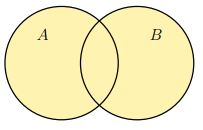
\includegraphics[width=50pt]{./images/vereinigung.jpg}
    \item Schnittmenge: $A \cup B := \{x\,|\,x \in A\, \land\, x \in B \}$
    \item 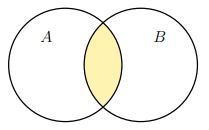
\includegraphics[width=50pt]{./images/schnittmenge.jpg}
    \item Differenz: $A \backslash B := \{x\,|\,x \in A\, \land\, x \notin B \}$
    \item 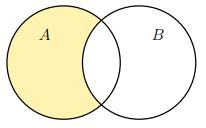
\includegraphics[width=50pt]{./images/differenz.jpg}
    \item Symmetrische Differenz: $A\Delta B := (A\backslash B)\cup (B\backslash A)$
    \item 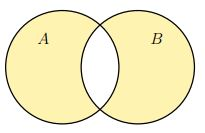
\includegraphics[width=50pt]{./images/systematische_differenz.jpg}
    \item Komplementierung (G Grundmenge): $\overline{A} := G\backslash A$
    \item 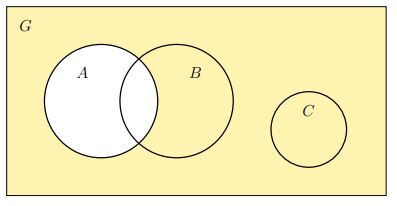
\includegraphics[width=80pt]{./images/komplementaer.jpg}
\end{itemize}
\vspace{1mm}

\paragraph{Mengen Rechenregeln}\mbox{}\\
\begin{tabularx}{\columnwidth}{@{}X|X@{}}
    \hline
    $B\cup A = A\cup B$                                              & $B\cap A = A \cap B$                                                      \\ \hline
    $(A\cup B)\cup C = A\cup (B\cup C)$                              & $(A\cap B)\cap C = A\cap (B\cap C)$                                       \\ \hline
    $A\cap (B\cup C) = (A\cap B)\cup (A\cap C)$                      & $A\cup (B\cap C) = (A\cup B)\cap (A\cup C)$                               \\ \hline
    $A\cup (A\cap B) = A$                                            & $A\cap (A\cup B) = A$                                                     \\ \hline
    $(A\backslash B)\backslash C = A \backslash (B\cup C)$           & $A\backslash (B\backslash C) = (A \backslash B)\cup (A\cap C)$            \\ \hline
    $(A\cup B) \backslash C = (A \backslash C) \cup (B\backslash C)$ & $(A\cap B) \backslash C = (A \backslash C) \cap (B \backslash C)$         \\ \hline
    $A\backslash (B\cup C) = (A \backslash B)\cap (A \backslash C)$  & $ A\backslash(B\cap C) = (A\backslash B) \cup (A \backslash C) $          \\ \hline
    $B\Delta A = A\Delta B$                                          & $(A\Delta B)\Delta C = A\Delta (B\Delta C)$                               \\ \hline
    $(A\Delta B)\cap C = (A\cap C)\Delta (B\cap C)$                  &                                                                           \\ \hline
    $\overline{A\cup B} = \overline{A}\cap \overline{B}$             & $\overline{A\cap B} = \overline{A}\cup \overline{B}$                      \\ \hline
    $\overline{A\cup B} = G\backslash (A\cup B) =$                   & $ = (G\backslash A) \cap (G\backslash B) = \overline{A}\cap \overline{B}$ \\ \hline
    $\overline{A\cap B} = G\backslash (A\cap B) =$                   & $ = (G\backslash A) \cup (G\backslash B) = \overline{A}\cup \overline{B}$ \\ \hline
\end{tabularx}
\vspace{1mm}

\noindent
\textit{Kartesisches Produkt}\linebreak
\fbox{$A\, \times B := \{(x;y)\, |\, x \in A\, und\, y \in B\}$}
\vspace{1mm}

\paragraph{Zahlenmenge}\mbox{}\\
\begin{tabularx}{\columnwidth}{@{}X|X@{}}
    \hline
    $\mathbb{N}$: natürlichen Zahlen & $\mathbb{N}_0$: natürlichen Zahlen mit die Zahl 0 \\ \hline
    $\mathbb{Z}$: ganze Zahlen       & $\mathbb{Q}$: rationale Zahlen                    \\ \hline
    $\mathbb{R}$: reelle Zahlen      & $\mathbb{C}$: Komplexe Zahlen                     \\ \hline
\end{tabularx}
\vspace{1mm}

\paragraph{Intervalle}\mbox{}\\
\begin{tabularx}{\columnwidth}{@{}X|X@{}}
    \hline
    [a,b] = $\{x \in \mathbb{R} | a \leq  x \leq b \}$ & ]a,b] = $\{x \in \mathbb{R} | a < x \leq b \}$ \\ \hline
    [a,b[ = $\{x \in \mathbb{R} | a \leq  x < b \}$    & ]a,b[ = $\{x \in \mathbb{R} | a < x < b \}$    \\ \hline
    $\mathbb{R}^{+}_0 = [0,\infty]$                    & $\mathbb{R}^{+} = ]0,\infty]$                  \\ \hline
\end{tabularx}
\vspace{1mm}

\paragraph{Körperaxiome}\mbox{}\\
\noindent
Addition\linebreak
\begin{tabularx}{\columnwidth}{@{}X|X@{}}
    \hline
    Assoziativgesetz      & $x+(y+z) = (x+y)+z$                                                  \\ \hline
    Kommutativgesetz      & $x+y = y+x$                                                          \\ \hline
    Existenz der Null     & $\exists$ eine Zahl 0 $\in \mathbb{R}$:\linebreak $0+x=x, \forall x$ \\ \hline
    Existenz der Negation & $\forall x\exists -x$: $x+(-x) = 0$                                  \\ \hline
\end{tabularx}
\vspace{1mm}
\noindent
Multiplikation\linebreak
\begin{tabularx}{\columnwidth}{@{}X|X@{}}
    \hline
    Assoziativgesetz      & $x*(y*z) = (x*y)*z$                               \\ \hline
    Kommutativgesetz      & $x*y = y*x$                                       \\ \hline
    Existenz der Eins     & $\exists (1\in \mathbb{R}) \land 1 \neq 0: 1*x=x$ \\ \hline
    Existenz der Inversen & $\forall x \neq 0, \exists x^{-1}: x*x^{-1}=1$    \\ \hline
    Distributivgesetz     & $x*(y+z) = x*y + x*z = 1$                         \\ \hline
\end{tabularx}
\vspace{1mm}

\paragraph{Funktionen}\mbox{}\\
\begin{tabularx}{\columnwidth}{@{}X|X@{}}
    \hline
    $f : A \rightarrow B$                           & $x \rightarrow f(x) := Kondition$   \\ \hline
    $f : \{3,4\} \rightarrow \{5,6,7\}$             & $x \rightarrow f(x) := x + 2$       \\ \hline
    $f$: Funktionsname                              & $A$: Definitionsmenge               \\ \hline
    $B$: Zielmenge                                  & $x$: unabhängige Variable, Argument \\ \hline
    $f(x)$: abhängige Variable, Funktionswert                                             \\ \hline
    $f(y)^{-1}: Umkehrfunktion$                                                           \\ \hline
    Identität ist die Funktion zwischen zwei Mengen & $id_A : B \rightarrow A$            \\ \hline
\end{tabularx}
\vspace{1mm}

\paragraph{Bild und Urbild}\mbox{}\\
Seien A und B zwei Mengen, $f: A \rightarrow B$ eine Funktion und $\overline{A} \subseteq A$ sowie $\overline{B} \subseteq B$.
\begin{itemize}
    \item Bild: $f(\overline{A}) \subseteq B$
    \item Urbild: $f^{-1}(\overline{B}) \subseteq A$
\end{itemize}
\vspace{1mm}

\paragraph{Surjektiv}\mbox{}\\
\begin{itemize}
    \item Zu jedem $y\in B$ aus dem Zielbereich mindestens ein $x\in A$ aus dem Definitionsbereich
    \item f heisst surjektiv: $\forall y \in B, \forall x \in A$
    \item $y= f(x)$
    \item Beweis: $y = f(x)$
    \item 1. Nach x auflösen
    \item 2. Ausdruck hängt von y ab
    \item 3. Überprüfen, ob dieser Ausdruck für alle y aus $y\in B$ definiert ist und ein Teil von A ist
\end{itemize}
\vspace{1mm}

\paragraph{Injektiv}\mbox{}\\
\begin{itemize}
    \item Für jedes Element $y\in B$ höchstens ein Element $x\in A$ wobei $f(x)=y$
    \item Annahme: $f(x_1) = f(x_2)$, Ziel: $x_1 = x_2$
\end{itemize}
\vspace{1mm}

\paragraph{Reihen und Folgen}\mbox{}\\
\begin{itemize}
    \item \fbox{$a: \mathbb{N}\rightarrow B$,  $n \rightarrow a(n)$}
    \item Arithmetische Folge, $\forall c \in \mathbb{R},$ so dass $\forall k \in \mathbb{N}^{+}$
    \item $a_{k+1} = a_{k} + c$
    \item Geometrische Folge, $\forall c \in \mathbb{R},$ so dass $\forall k \in \mathbb{N}^{+}$
    \item $a_{k+1} = a_{k} * c$
    \item Arithmetische Folge ist die diskrete Version einer linearen Funktion:
    \item $a_n = a_0 + c * n$
    \item Geometrische Folge ist die diskrete Version einer Exponentialfunktion:
    \item $a_n= a_0 * c^n$ \\
\end{itemize}
\vspace{1mm}

\paragraph{Beschrankte Folgen}\mbox{}\\
\begin{itemize}
    \item Oben beschränkt: \fbox{$a_n \leq a_O$}
    \item Unten beschränkt: \fbox{$a_n \geq a_U$}
    \item Die folge $a_n$ heisst beschränkt wenn: \fbox{$a_n \in [a_U,a_O]$}
\end{itemize}
\vspace{1mm}

\paragraph{Monotone Folgen}\mbox{}\\
\begin{itemize}
    \item Monoton steigend: \fbox{$a_{k+1} \geq a_k $}
    \item Monoton streng steigend: \fbox{$a_{k+1} > a_k $}
    \item Monoton fallend: \fbox{$a_{k+1} \leq a_k $}
    \item Monoton streng fallend: \fbox{$a_{k+1} < a_k $}
\end{itemize}
\vspace{1mm}

\paragraph{Monotonie untersuchen}\mbox{}\\
\begin{itemize}
    \item Um eine Folge auf Monotonie zu untersucen, kann man die Folgeglieder der Differenzenfolge gegen Null abschätzen
    \item \fbox{$d_n := a_{n+1} - a_{n}$}
    \item Resultat interpretieren:
    \item $d_n \geq 0 \leftrightarrow a_{n+1} \geq a_n \leftrightarrow a_n$ ist monoton steigend
    \item $d_n > 0 \leftrightarrow a_{n+1} > a_n \leftrightarrow a_n$ ist streng monoton steigend
    \item $d_n \leq 0 \leftrightarrow a_{n+1} \leq a_n \leftrightarrow a_n$ ist monoton fallend
    \item $d_n < 0 \leftrightarrow a_{n+1} < a_n \leftrightarrow a_n$ ist streng monoton fallend
\end{itemize}
\vspace{1mm}

\paragraph{Konvergenz und Divergenz}\mbox{}\\
\begin{itemize}
    \item $|a_{n} - G| \leq \epsilon $
    \item G steht für Grenzwert
    \item Die Folgen können mit dem Pfeil angegeben werden, bei welchen der n gegen irgendwas tendiert.
    \item $a_n = ... = ... \xrightarrow{n \rightarrow \infty}$
    \item WICHTIG: Eine Folge kann \textbf{nicht} nach $\infty$ oder $-\infty$ konvergieren.
    \item WICHTIG: Eine Folge kann nur konvergieren, nur divergieren oder beides, jedoch in verschiedene Richtungen.
    \item WICHTIG: Eine Folge divergiert nur gegen $\infty$ oder $-\infty$, jedoch nicht zur einer Zahl.
    \item Um die untere Grenze zu bestimmen, muss der Vergleichsterm kleiner sein als die Folge. Meistens wird der Nenner erhöht.
    \item Bsp: $a_n := \underbrace{\frac{n+2}{n+1}}_{Folge} \geq \underbrace{\frac{n+2}{n+2}}_{Vergleichsterm} = 1 := a_U$
    \item Um die obere Grenze zu bestimmen, muss der Vergleichsterm grösser sein als die Folge. Meistens wird der Zähler erhöht.
    \item Bsp: $a_n := \underbrace{\frac{n+2}{n+1}}_{Folge} \leq \underbrace{\frac{2n+2}{n+1}}_{Vergleichsterm} = \frac{2 \cdot (n+1)}{n+1} = 2 := a_O$
\end{itemize}
\vspace{1mm}

\paragraph{Grenzwertsätze und Rechenregeln}\mbox{}\\
\noindent
\begin{tabularx}{\columnwidth}{@{}X@{}}
    \hline
    \[ \lim_{n \to \infty} (a_n \pm b_n ) = \lim_{n \to \infty} a_n \pm \lim_{n \to \infty} b_n \]       \\ \hline
    \[ \lim_{n \to \infty} (a_n \cdot b_n ) = \lim_{n \to \infty} a_n \cdot \lim_{n \to \infty} b_n \]   \\ \hline
    \[ \lim_{n \to \infty}  \frac{a_n}{b_n} = \frac{lim_{n \to \infty} a_n}{\lim_{n \to \infty} b_n} \]  \\ \hline
    \[ \lim_{n \to \infty} a_n^{b_n} = \left( lim_{n \to \infty} a_n\right)^{\lim_{n \to \infty} b_n} \] \\ \hline
\end{tabularx}
\vspace{1mm}

\paragraph{Grenzwert-Rechenregeln mit einer Konstanten}\mbox{}\\
\noindent
\begin{tabularx}{\columnwidth}{@{}X@{}}
    \hline
    \[ \lim_{n \to \infty} p = p \]                                             \\ \hline
    \[ \lim_{n \to \infty} (a_n \pm p ) = \lim_{n \to \infty} a_n \pm p \]      \\ \hline
    \[ \lim_{n \to \infty} (a_n \cdot p ) = \lim_{n \to \infty} a_n\cdot p \]   \\ \hline
    \[ \lim_{n \to \infty} \frac{p}{a_n} = \frac{p}{\lim_{n \to \infty} a_n} \] \\ \hline
    \[ \lim_{n \to \infty} a_n^p = (\lim_{n \to \infty} a_n)^p \]               \\ \hline
    \[ \lim_{n \to \infty} p^{a_n} = p^{\lim_{n \to \infty} a_n} \]             \\ \hline
\end{tabularx}
\vspace{1mm}

\paragraph{Rechenregeln für Summen}\mbox{}\\
\noindent
\begin{tabularx}{\columnwidth}{@{}X@{}}
    \hline
    Seien $m,n,p \in \mathbb{Z}$ mit $m\leq n,C \in \mathbb{R}$ und $f: \mathbb{Z} \to \mathbb{R}$ eine Funktion, dann gelten die folgende Regeln. \\
    Distributivgesetz                                                                                                                              \\
    \[ \sum_{k=m}^n C \cdot f(k) = C \cdot \sum_{k=m}^n f(k) \]                                                                                    \\ \hline
    Verschiebungsgesetz                                                                                                                            \\
    \[ \sum_{k=m}^n f(k) = C \cdot \sum_{k=m\pm p}^{n\pm p} f(k\mp p) \]                                                                           \\ \hline
    Anzahl Summanden in heder Summe von m bis n beträgt:
    \[ N = (n - m + 1) \]                                                                                                                          \\ \hline
    Geometrische Summe                                                                                                                             \\
    \[ G_{(m;n)}(x) := \sum_{k=m}^n x^k = x^m + x^{m+1} + ... + x^n \]                                                                             \\ \hline
\end{tabularx}
\vspace{1mm}

\paragraph{Rechenregeln für Summen}\mbox{}\\
\noindent
\begin{tabularx}{\columnwidth}{@{}X@{}}
    \hline
    Geometrische Summen-Formel                                                                    \\
    \[ G_{(m;n)}(x) := \sum_{k=m}^n x^k = \frac{x^m - x^{n+1}}{1-x} \]                            \\ \hline
    Geometrische Reihe                                                                            \\
    \[ \sum_{k=m}^\infty x^k = \lim_{n\to\infty} \sum_{k=m}^n x^k = \begin{cases} \frac{x^m}{1-x} | x \in [-1,1[ \\ divergent | x \notin [-1,1[ \end{cases} \] \\ \hline
\end{tabularx}
\vspace{1mm}

\paragraph{Rechenregeln für Summen}\mbox{}\\
\noindent
\begin{tabularx}{\columnwidth}{@{}X|X@{}}
    \hline
    Basler-Reihen                                                                                                                                                \\
    \[ \sum_{k=1}^n \frac{1}{k} \xrightarrow{n\to\infty} \infty \]         & \[ \sum_{k=1}^n \frac{1}{k^2} \xrightarrow{n\to \infty} \frac{\pi^2}{6} \]          \\ \hline
    \[ \sum_{k=1}^n \frac{(-1)^{k+1}}{k} \xrightarrow{n\to\infty} ln(2) \] & \[ \sum_{k=1}^n \frac{(-1)^{k+1}}{k^2} \xrightarrow{n\to\infty} \frac{\pi^2}{12} \] \\ \hline
\end{tabularx}
\vspace{1mm}

\paragraph{Winkel}\mbox{}\\
\noindent
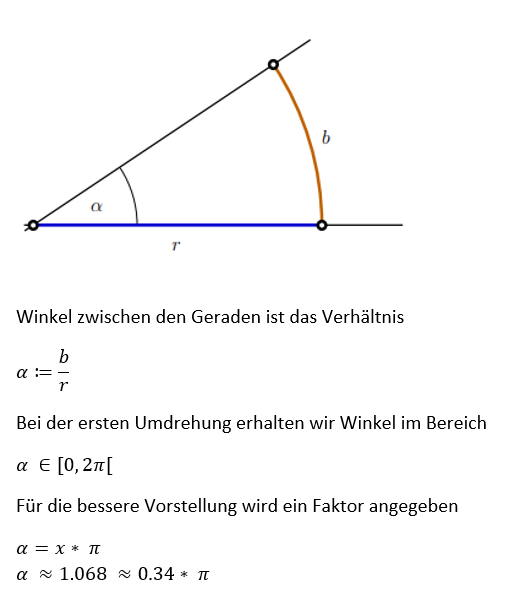
\includegraphics[width=\columnwidth]{./images/winkel.png}
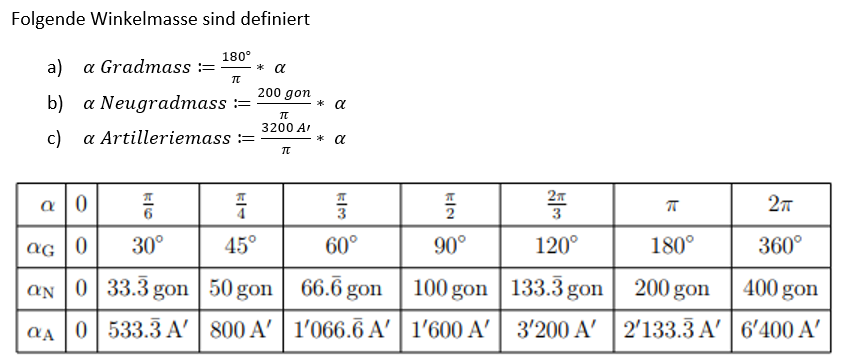
\includegraphics[width=\columnwidth]{./images/winkel1.png}
\vspace{1mm}

\paragraph{Lineare Gleichungssysteme}\mbox{}\\
\noindent
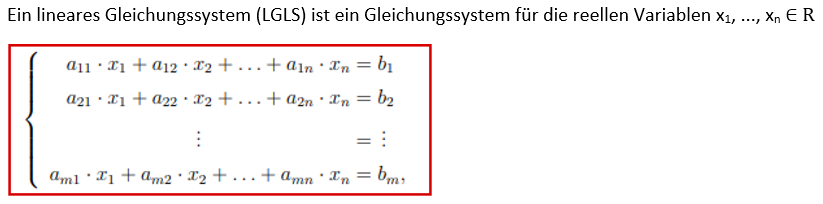
\includegraphics[width=\columnwidth]{./images/lgs1.png}
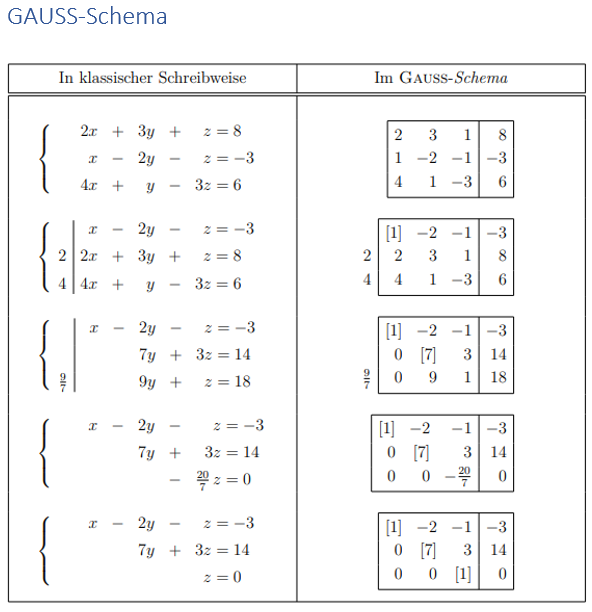
\includegraphics[width=\columnwidth]{./images/lgs2.png}
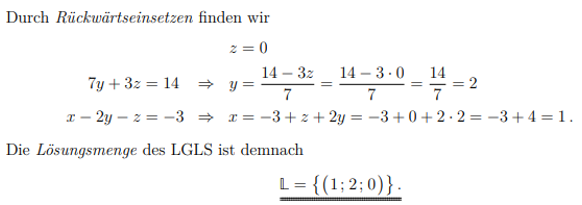
\includegraphics[width=\columnwidth]{./images/lgs3.png}
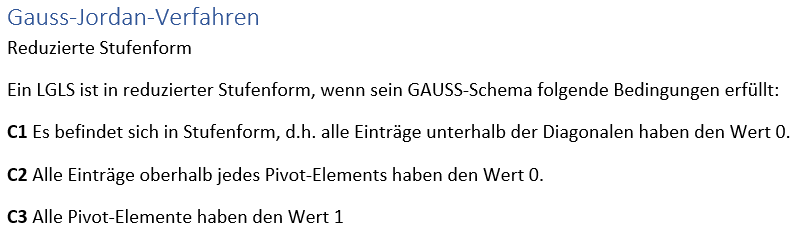
\includegraphics[width=\columnwidth]{./images/lgs4.png}
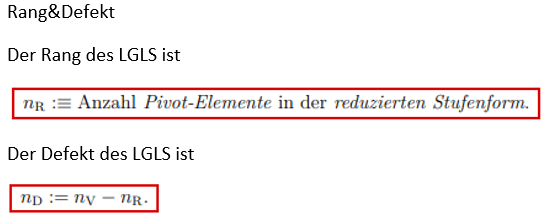
\includegraphics[width=\columnwidth]{./images/lgs5.png}
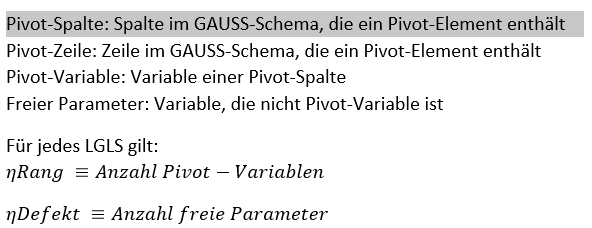
\includegraphics[width=\columnwidth]{./images/lgs6.png}
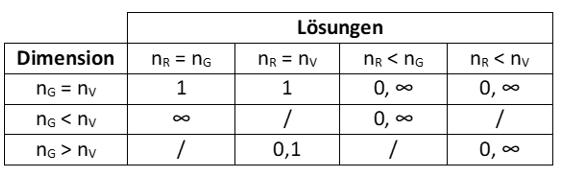
\includegraphics[width=\columnwidth]{./images/lgs7.png}
\vspace{1mm}

\paragraph{Elementarfunktionen}\mbox{}\\
\noindent
\begin{tabularx}{\columnwidth}{@{}X@{}}
    \hline
    Eine reele Funktion ist eine Funktion der Form $f: A \to B$                         \\
    \[ f: \mathbb{R} \to \mathbb{R},x \rightarrow f(x) = 3 \cdot x^2 + 5 \cdot x + 7 \] \\
\end{tabularx}
\begin{tabularx}{\columnwidth}{@{}X|X|X@{}}
    Oben beschränkt & Unten beschränkt & Beschränkt           \\
    $f(x) \leq y_O$ & $f(x) \geq y_U$  & $f(x) \in [y_U,y_O]$ \\ \hline
\end{tabularx}
\vspace{1mm}

\paragraph{Monotone Funktionen}\mbox{}\\
\noindent
\begin{tabularx}{\columnwidth}{@{}X|X@{}}
    \hline
    Monoton steigend        & $x_1 < x_2 \rightarrow f(x_1) \leq f(x_2)$ \\ \hline
    Streng Monoton steigend & $x_1 < x_2 \rightarrow f(x_1) < f(x_2)$    \\ \hline
    Monoton fallend         & $x_1 > x_2 \rightarrow f(x_1) \geq f(x_2)$ \\ \hline
    Streng Monoton fallend  & $x_1 > x_2 \rightarrow f(x_1) > f(x_2)$    \\ \hline
\end{tabularx}
\vspace{1mm}

\paragraph{Betragsfunktion (Absolute)}\mbox{}\\
\noindent
\begin{tabularx}{\columnwidth}{@{}XX@{}}
    \hline
    \fbox{$abs: \mathbb{R} \to \mathbb{R}_0^+$}
    \fbox{$ x \rightarrow abs(x) := |x| = \begin{cases} -x | x < 0 \\ 0 | x = 0 \\ x | x > 0 \end{cases} $}
    \begin{tikzpicture}
        \begin{axis}[
                xlabel=$x$,
                ylabel={$ y = |x|$},
                axis lines=middle
            ]
            \addplot {abs(x)};
        \end{axis}
    \end{tikzpicture} \\
\end{tabularx}

\paragraph{Ableitung der Betragsfunktion für x}\mbox{}\\
\noindent
\begin{tabularx}{\columnwidth}{@{}X@{}}
    \hline
    \[ abs(x)' = sgn(x) \] \\ \hline
\end{tabularx}
\vspace{1mm}

\tikzset{
    declare function={
            sgn(\x) = (and(\x<0, 1) * -1) +
            (and(\x>0, 1) * 1);
        }
}

\paragraph{Vorzeichenfunktion (Signum)}\mbox{}\\
\noindent
\begin{tabularx}{\columnwidth}{@{}XX@{}}
    \hline
    \fbox{$sgn: \mathbb{R} \to \lbrace-1,0,1\rbrace$}
    \fbox{$ x \rightarrow sgn(x) := |x| = \begin{cases} -1 | x < 0 \\ 0 | x = 0 \\ +1 | x > 0 \end{cases} $}
    \begin{tikzpicture}
        \begin{axis}[
                axis lines=middle,
                xlabel=$x$,
                ylabel={$y$},
                xmin=-3, xmax=3,
                ymin=-1.5, ymax=1.5,
                xtick=\empty,
                ytick={0, 1},
                extra y ticks={-1},
                extra y tick style={
                        tick label style={anchor=west, xshift=3pt},
                    },
            ]
            \addplot[red, mark=*] coordinates {(0, 0)};
            \addplot[
                mark=*,
                mark options={fill=white, draw=black},
                only marks,
            ] coordinates {(0, -1) (0, 1)};
            \addplot[red, thick, samples=1000,
                domain=0.001:\pgfkeysvalueof{/pgfplots/xmax}]
            {sign(x)};
            \addplot[red, thick, samples=1000,
                domain=\pgfkeysvalueof{/pgfplots/xmin}:-0.001]
            {sign(x)};
        \end{axis}
    \end{tikzpicture} \\
    Dreiecksungleichung \fbox{$|x \pm y| \leq |x| + |y|$}
\end{tabularx}

\paragraph{Eigentliche Exponentialfunktion}\mbox{}\\
\noindent
\begin{tabularx}{\columnwidth}{@{}XX@{}}
    \hline
    Die Funktionswerte von eigentlichen Exponentialfunktionen sind strikt positive. Mit der Bildmenge R+ als Zielmenge sind eigentliche Exponentialfunktionen sogar bijektiv. \\
    \fbox{$\mathbb{R}\to\mathbb{R}^+$} & \fbox{$x \to f(x) := a^x$}                                                                                                           \\ \hline
    \fbox{$f(0) = 1$ und $f(x + 1) = a \cdot f(x)$}
\end{tabularx}
\vspace{1mm}

\paragraph{Trigonometrische Funktionen}\mbox{}\\
\noindent
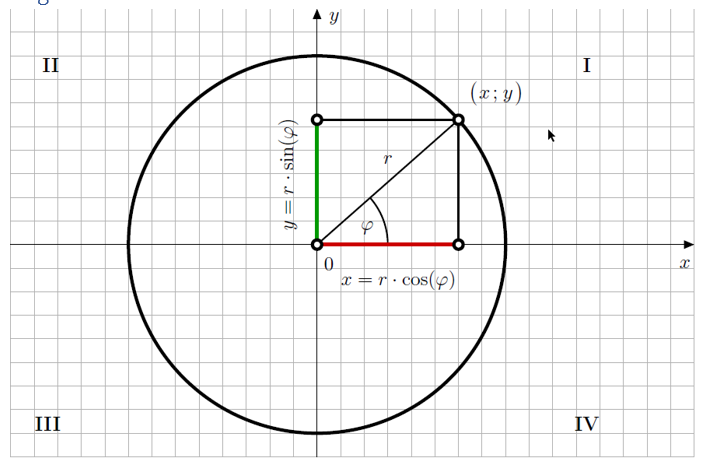
\includegraphics[width=\columnwidth]{./images/trigo_circle.png}
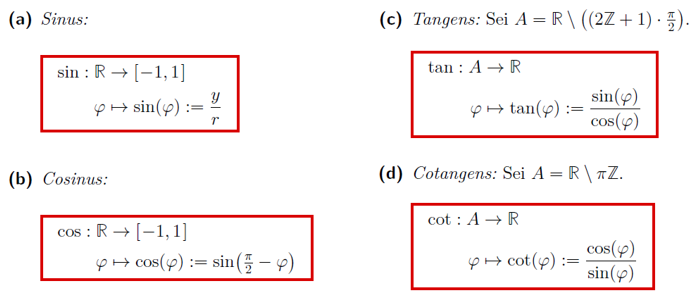
\includegraphics[width=\columnwidth]{./images/trigo_circle1.png}
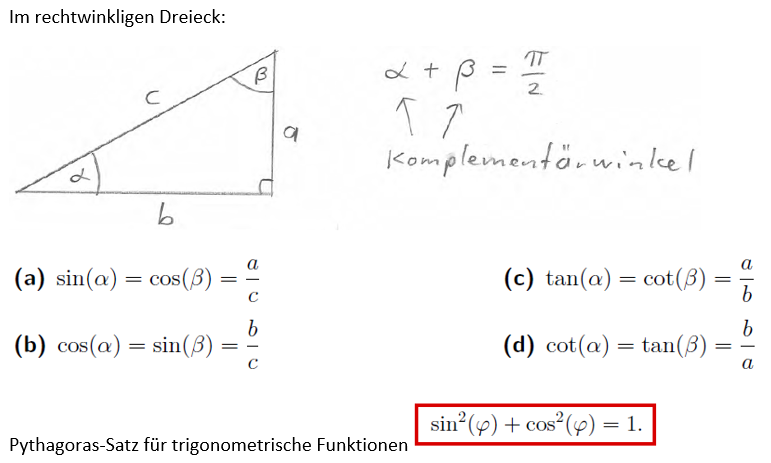
\includegraphics[width=\columnwidth]{./images/trigo_circle2.png}
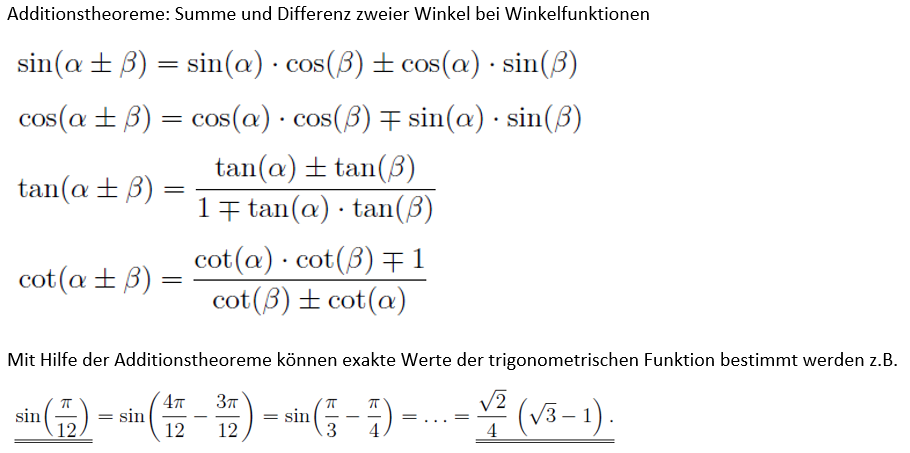
\includegraphics[width=\columnwidth]{./images/trigo_circle3.png}
\vspace{1mm}

\paragraph{Hyperbolische Funktionen}\mbox{}\\
\noindent
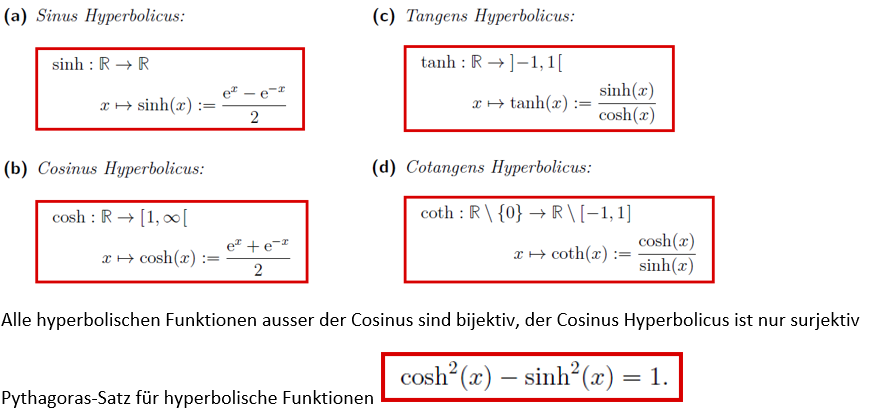
\includegraphics[width=\columnwidth]{./images/hyper.png}
\vspace{1mm}

\paragraph{Einfache Modifikation}\mbox{}\\
\noindent
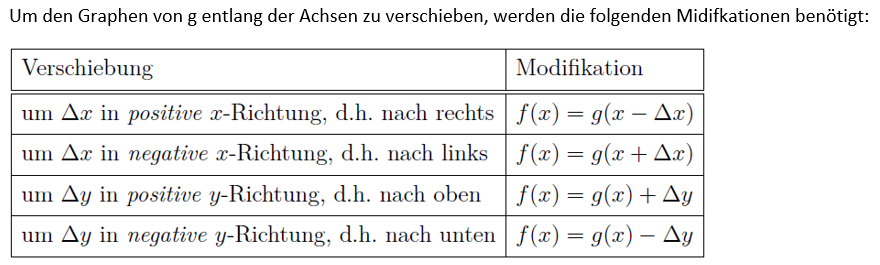
\includegraphics[width=\columnwidth]{./images/mod.png}
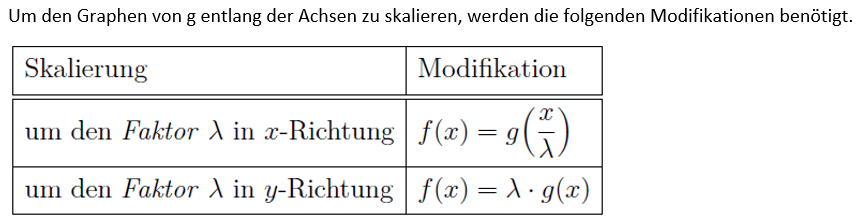
\includegraphics[width=\columnwidth]{./images/mod1.png}
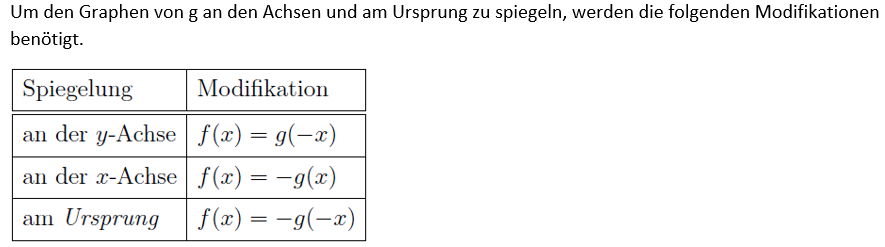
\includegraphics[width=\columnwidth]{./images/mod2.png}
\vspace{1mm}

\paragraph{Parität}\mbox{}\\
\noindent
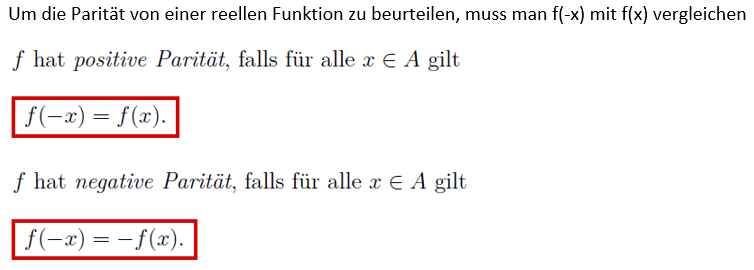
\includegraphics[width=\columnwidth]{./images/paritat.png}
\vspace{1mm}

\paragraph{Lineare Funktionen}\mbox{}\\
\noindent
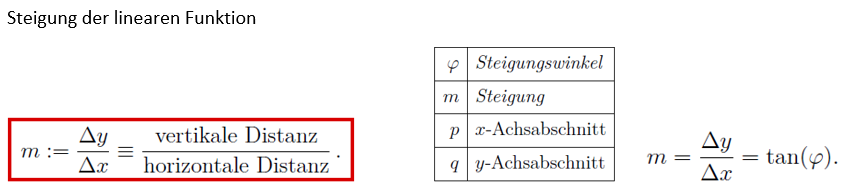
\includegraphics[width=\columnwidth]{./images/lin.png}
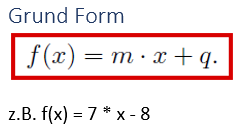
\includegraphics[width=\columnwidth]{./images/lin1.png}
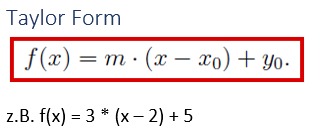
\includegraphics[width=\columnwidth]{./images/lin2.png}
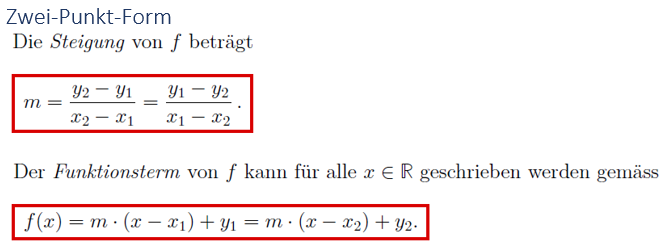
\includegraphics[width=\columnwidth]{./images/lin3.png}
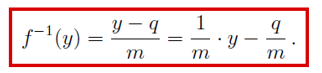
\includegraphics[width=\columnwidth]{./images/lin4.png}
\vspace{1mm}

\paragraph{Quadratische Funktionen}\mbox{}\\
\noindent
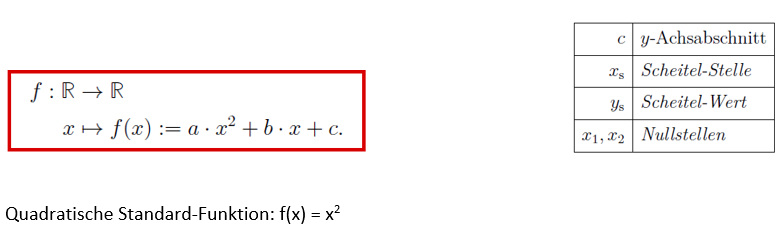
\includegraphics[width=\columnwidth]{./images/quad.png}
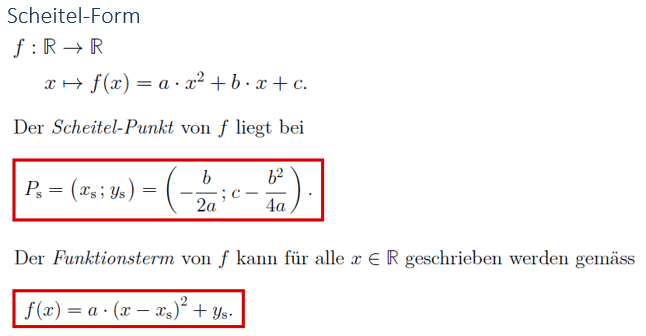
\includegraphics[width=\columnwidth]{./images/quad1.png}
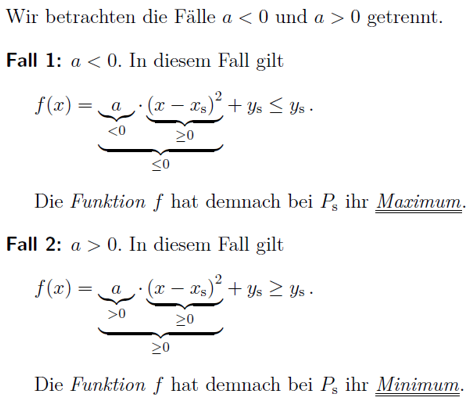
\includegraphics[width=\columnwidth]{./images/quad2.png}
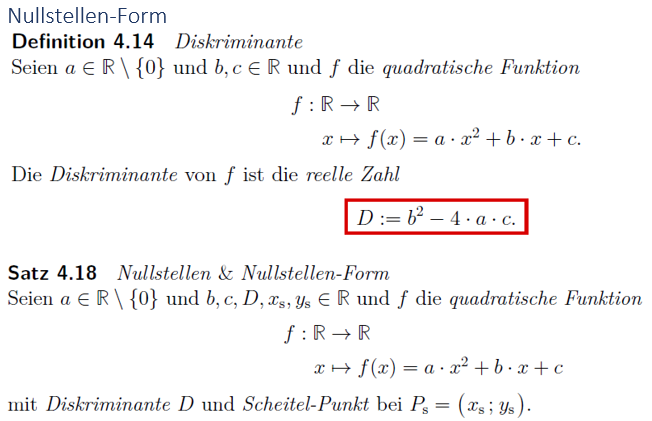
\includegraphics[width=\columnwidth]{./images/quad3.png}
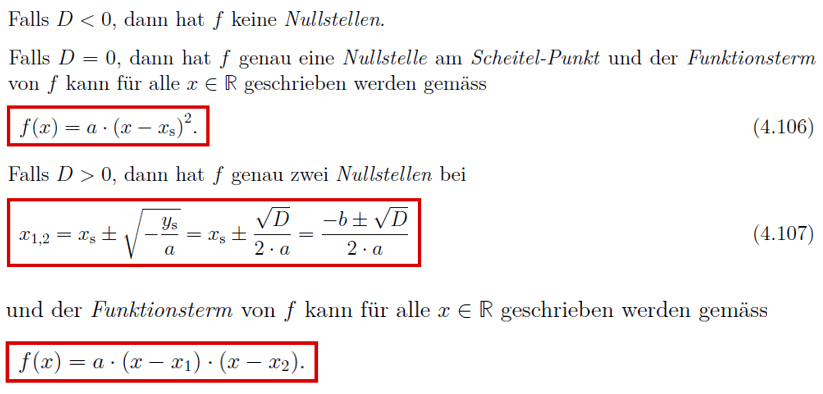
\includegraphics[width=\columnwidth]{./images/quad4.png}
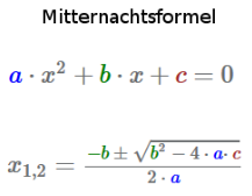
\includegraphics[width=\columnwidth]{./images/quad5.png}
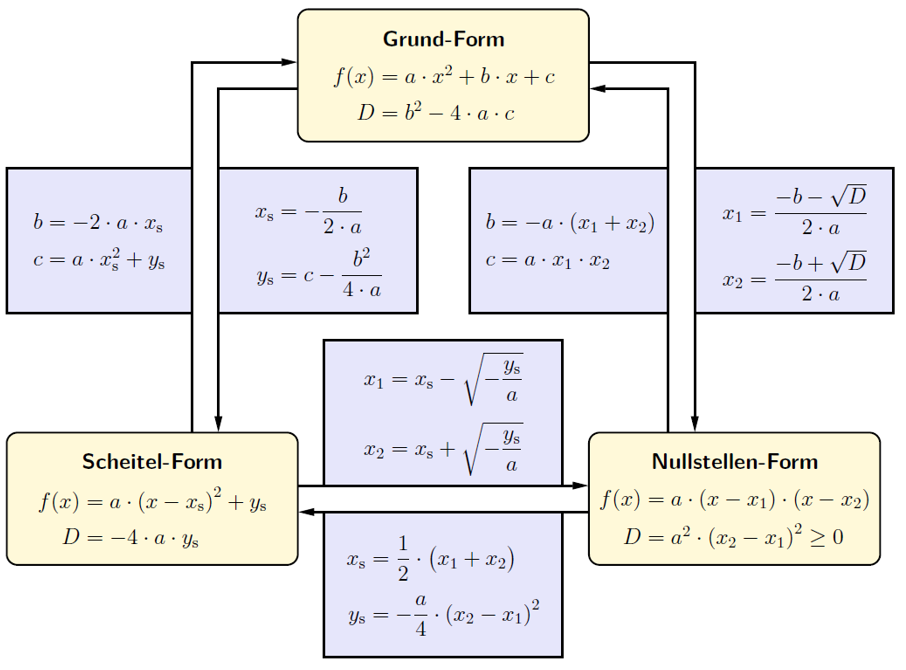
\includegraphics[width=\columnwidth]{./images/quad6.png}
\vspace{1mm}

\paragraph{Verallgemeinerte Exponentialfunktionen}\mbox{}\\
\noindent
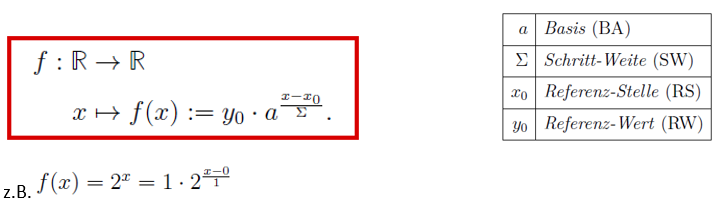
\includegraphics[width=\columnwidth]{./images/expo.png}
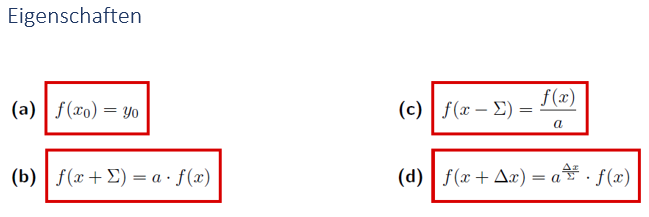
\includegraphics[width=\columnwidth]{./images/expo1.png}
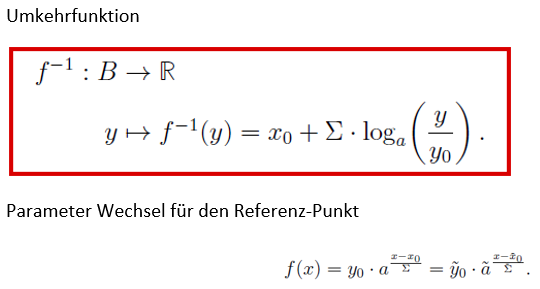
\includegraphics[width=\columnwidth]{./images/expo2.png}
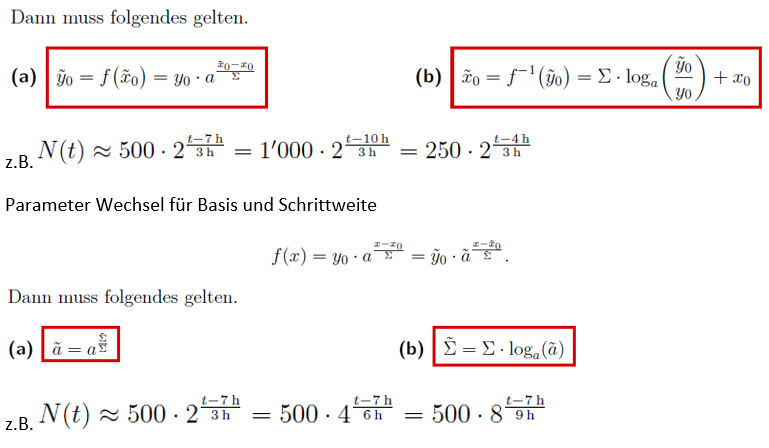
\includegraphics[width=\columnwidth]{./images/expo3.png}
\begin{tabularx}{\columnwidth}{@{}X@{}}
    \hline
    Schrittweite (Sigma) berrechnen                       \\
    \[ \frac{(x-x_0)*ln(a)}{ln(f(x))-ln(y_0)} = \Sigma \] \\ \hline
\end{tabularx}
\vspace{1mm}

\paragraph{Differentialgleichungen}\mbox{}\\
\noindent
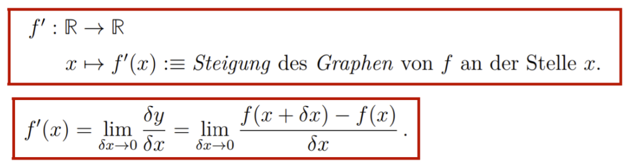
\includegraphics[width=\columnwidth]{./images/diff.png}
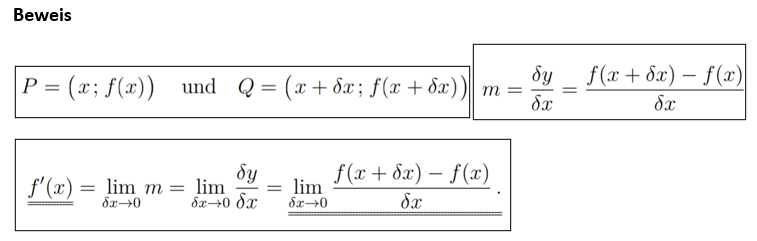
\includegraphics[width=\columnwidth]{./images/diff1.png}
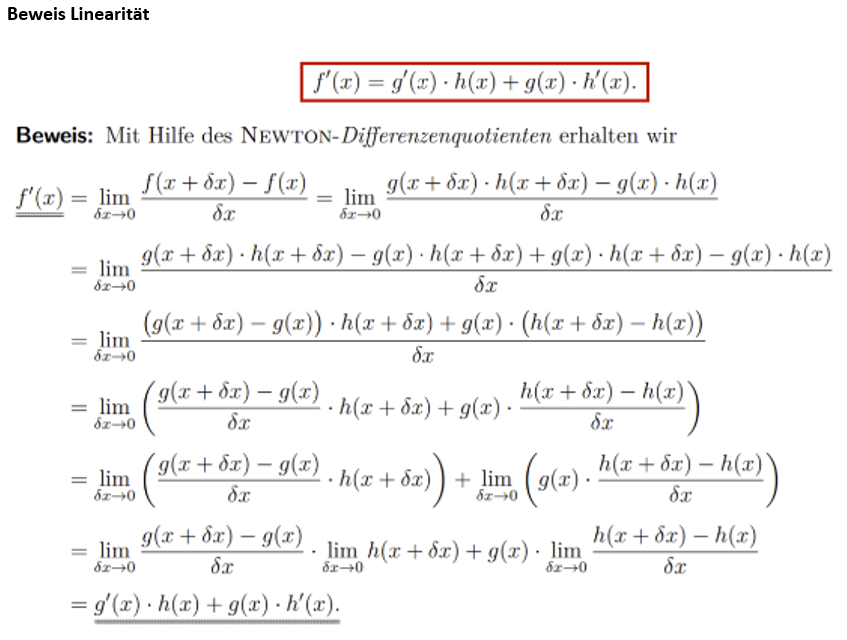
\includegraphics[width=\columnwidth]{./images/diff2.png}
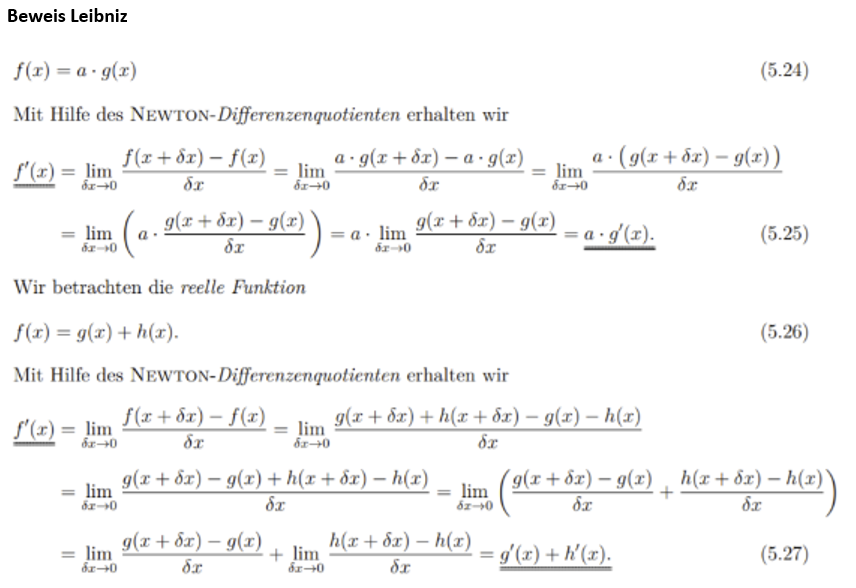
\includegraphics[width=\columnwidth]{./images/diff3.png}
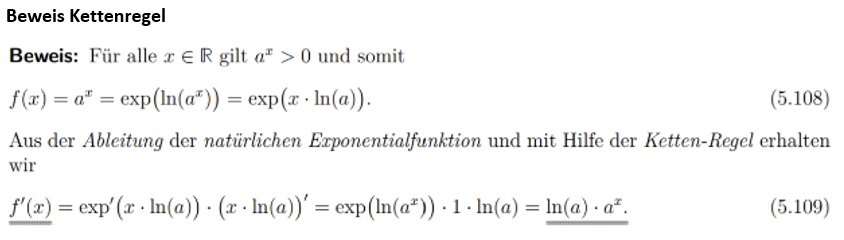
\includegraphics[width=\columnwidth]{./images/diff4.png}
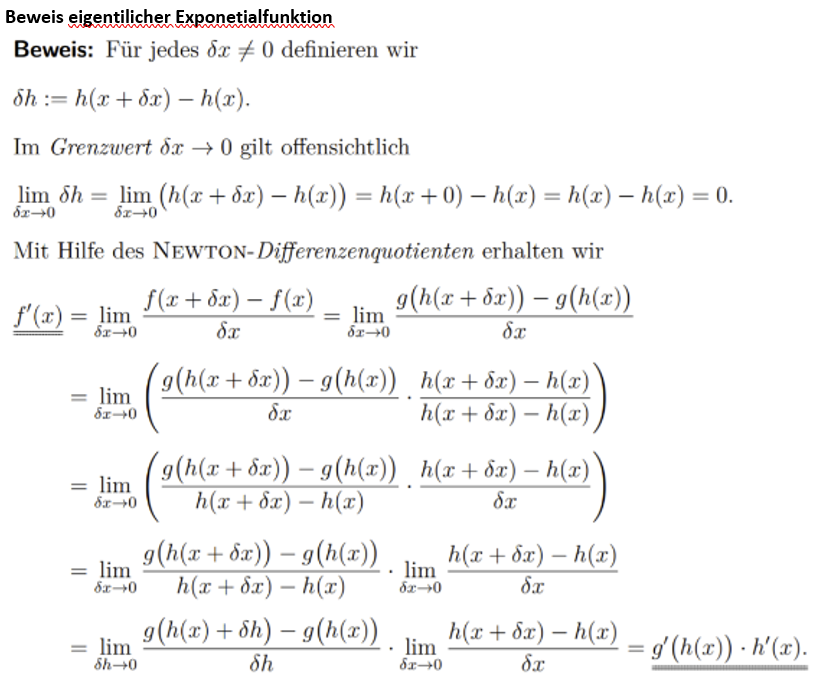
\includegraphics[width=\columnwidth]{./images/diff5.png}
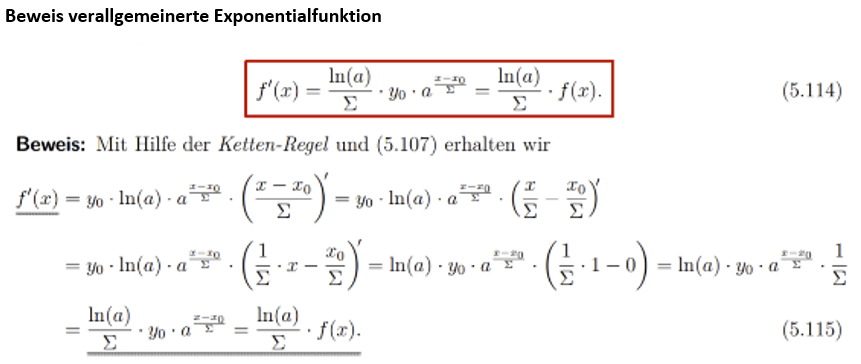
\includegraphics[width=\columnwidth]{./images/diff6.png}
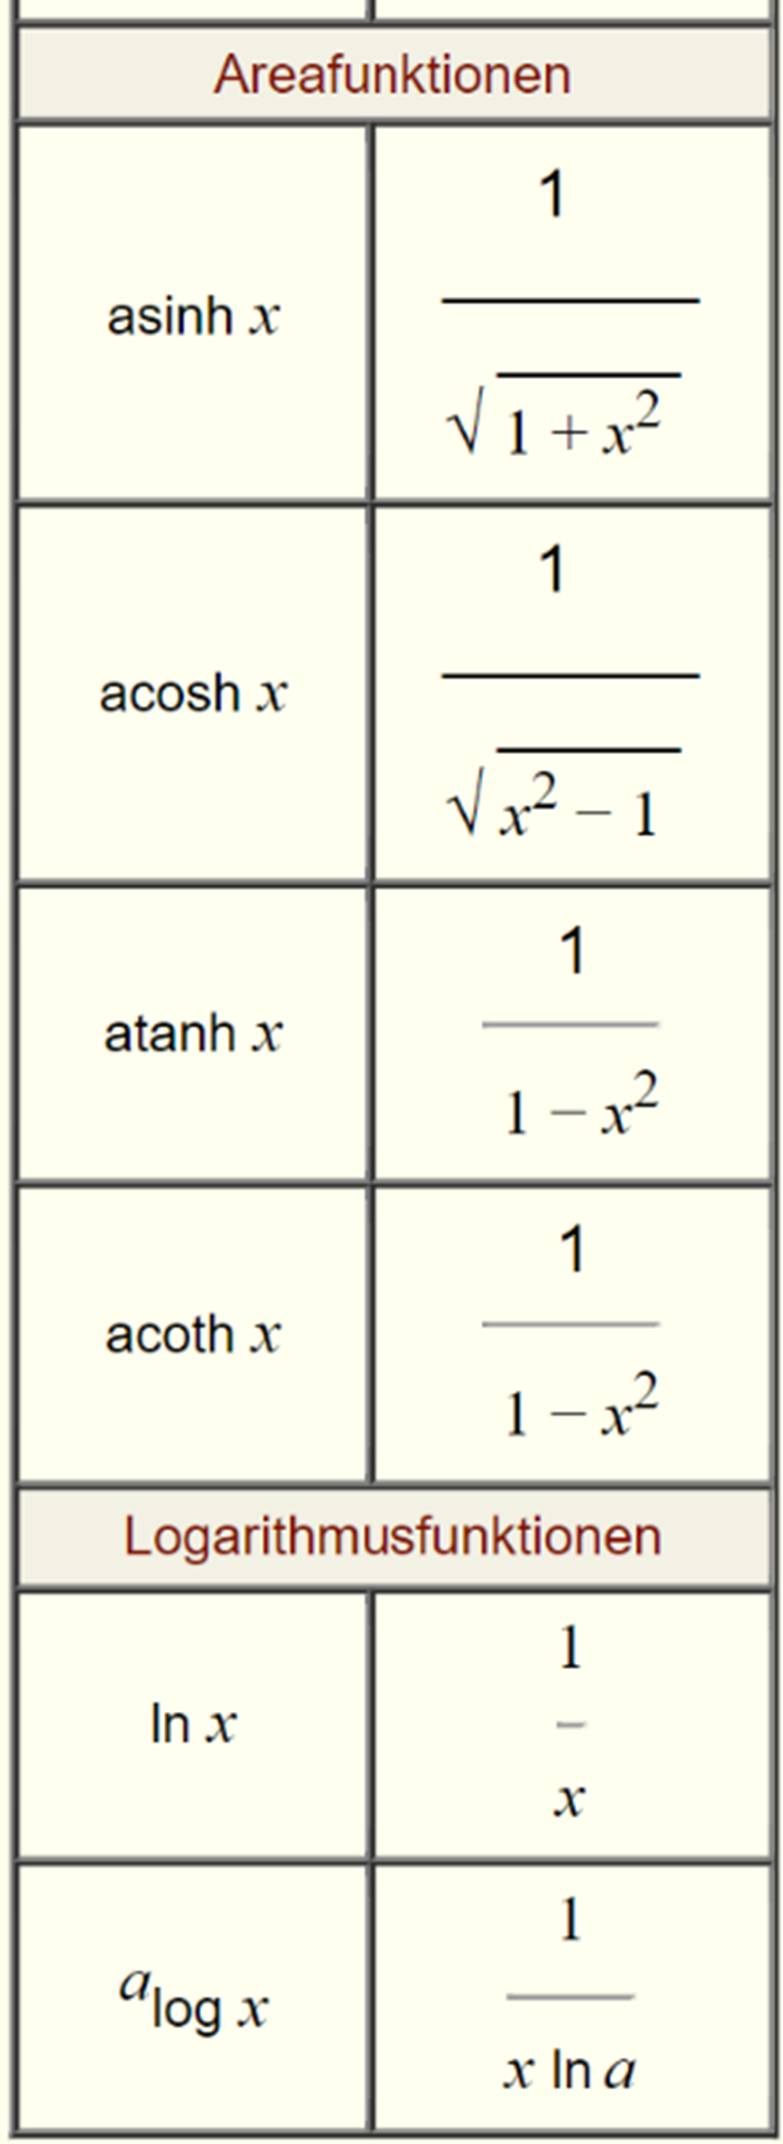
\includegraphics[width=\columnwidth]{./images/diff7.png}
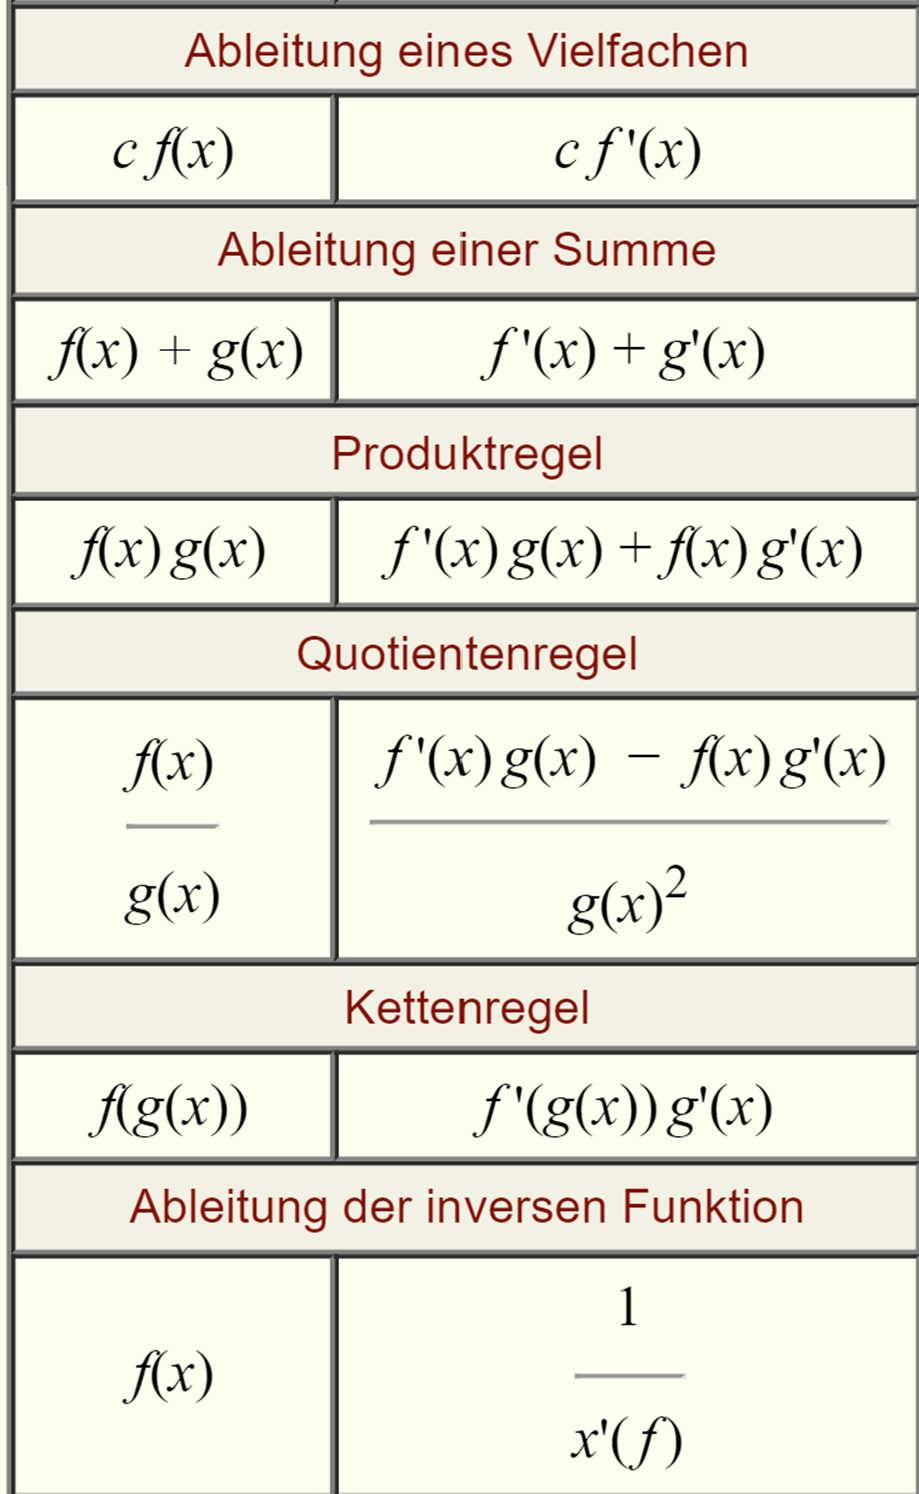
\includegraphics[width=\columnwidth]{./images/diff8.png}
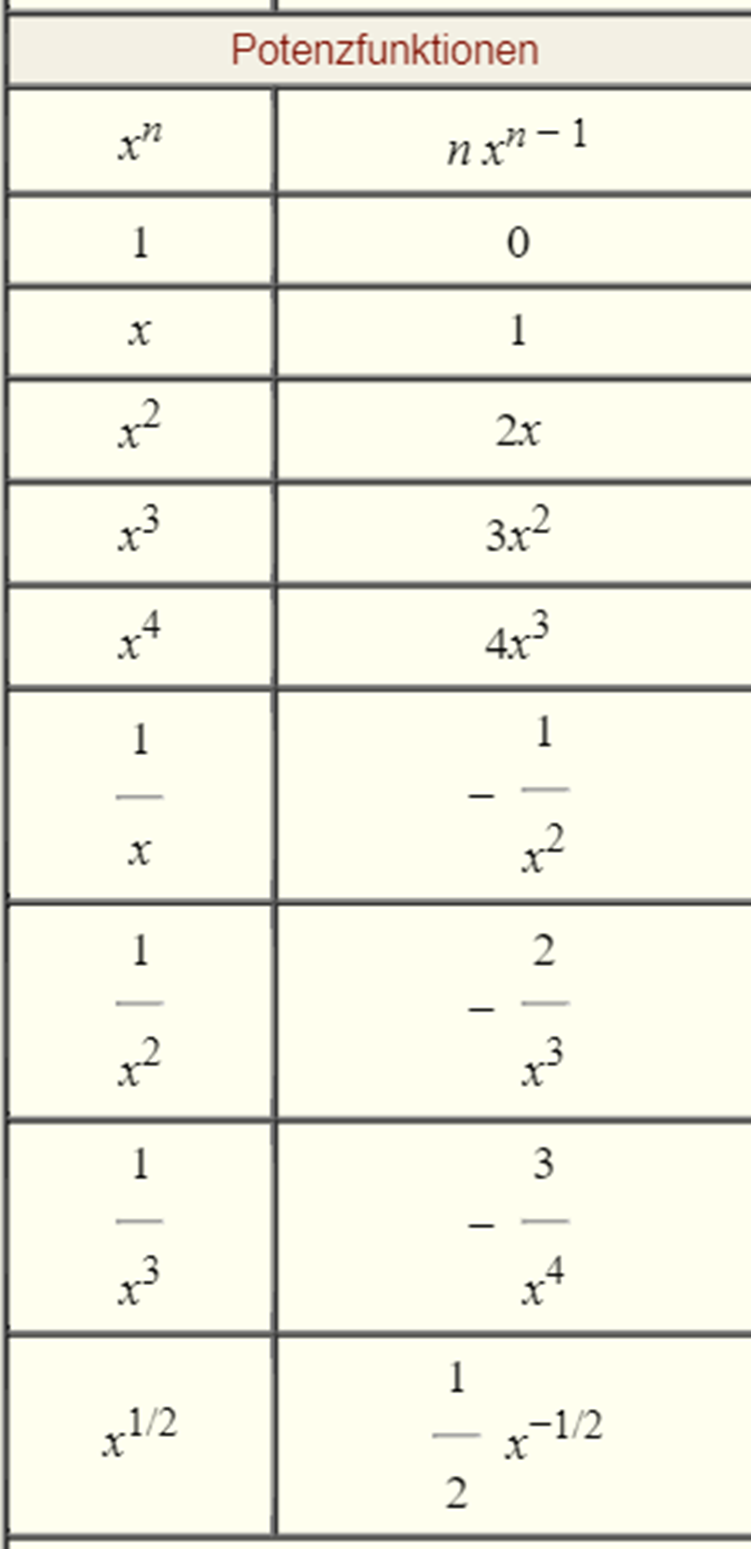
\includegraphics[width=\columnwidth]{./images/diff9.png}
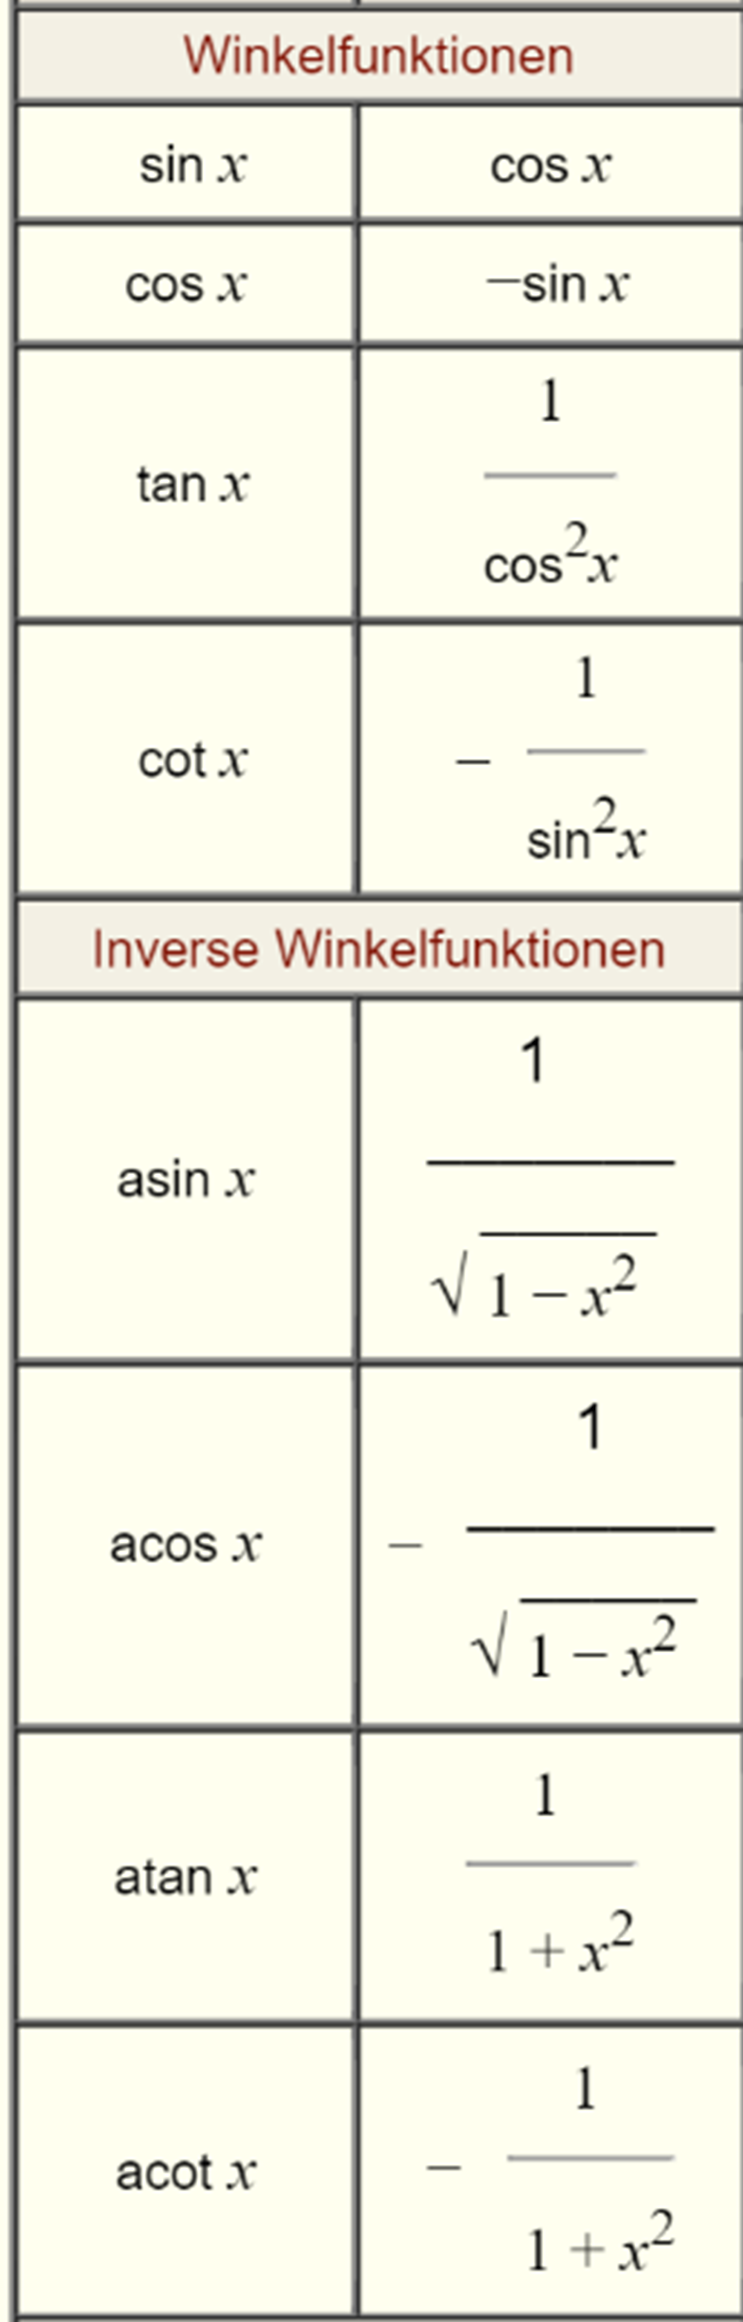
\includegraphics[width=\columnwidth]{./images/diff10.png}
\vspace{1mm}

\paragraph{Integralrechnung}\mbox{}\\
\noindent
\includegraphics[width=\columnwidth]{./images/int.png}
\includegraphics[width=\columnwidth]{./images/int1.png}
\includegraphics[width=\columnwidth]{./images/int2.png}
\includegraphics[width=\columnwidth]{./images/int3.png}
\includegraphics[width=\columnwidth]{./images/int4.png}
\vspace{1mm}

\paragraph{Kurvendiskussion}\mbox{}\\
\noindent
\includegraphics[width=\columnwidth]{./images/kurv.png}
\includegraphics[width=\columnwidth]{./images/kurv1.png}
\vspace{1mm}

\paragraph{Vektorgeometrie}\mbox{}\\
\noindent
\includegraphics[width=80pt]{./images/vek.png}\linebreak
\includegraphics[width=\columnwidth]{./images/vek1.png}
\includegraphics[width=\columnwidth]{./images/vek2.png}
\includegraphics[width=\columnwidth]{./images/vek3.png}
\includegraphics[width=\columnwidth]{./images/vek4.png}
\includegraphics[width=\columnwidth]{./images/vek5.png}
\includegraphics[width=\columnwidth]{./images/vek6.png}
\includegraphics[width=\columnwidth]{./images/vek7.png}
\includegraphics[width=\columnwidth]{./images/vek8.png}
\includegraphics[width=\columnwidth]{./images/vek9.png}
\includegraphics[width=\columnwidth]{./images/vek10.png}
\includegraphics[width=\columnwidth]{./images/vek11.png}
\paragraph{Spatprodut oder gemischtes Produkt}\mbox{}\\
\noindent
\begin{tabularx}{\columnwidth}{@{}X@{}}
    \hline
    $<\vec{u},\vec{v}\times\vec{w}>$ Spatprodukt                                                       \\
    - Zyklische Vertauschung erhält den Wert:                                                          \\
    $<\vec{u},\vec{v}\times\vec{w}> = <\vec{v},\vec{w}\times\vec{u}> = <\vec{w},\vec{u}\times\vec{v}>$ \\
    - Vertauschen zweier Vektoren ändert Vorzeichen:                                                   \\
    $<\vec{u},\vec{v}\times\vec{w}> = -<\vec{w},\vec{v}\times\vec{u}> $                                \\
\end{tabularx}
\includegraphics[width=\columnwidth]{./images/vek12.png}
\includegraphics[width=\columnwidth]{./images/vek13.png}
\includegraphics[width=\columnwidth]{./images/vek14.png}
\includegraphics[width=\columnwidth]{./images/vek15.png}
\includegraphics[width=\columnwidth]{./images/vek16.png}
\includegraphics[width=\columnwidth]{./images/vek17.png}
\includegraphics[width=\columnwidth]{./images/vek18.png}
\includegraphics[width=\columnwidth]{./images/vek19.png}
\includegraphics[width=\columnwidth]{./images/vek20.png}
\includegraphics[width=\columnwidth]{./images/vek21.png}
\includegraphics[width=\columnwidth]{./images/vek22.png}
\includegraphics[width=\columnwidth]{./images/vek23.png}
\includegraphics[width=\columnwidth]{./images/vek24.png}
\includegraphics[width=\columnwidth]{./images/vek25.png}
\includegraphics[width=\columnwidth]{./images/vek26.png}
\includegraphics[width=\columnwidth]{./images/vek27.png}
\includegraphics[width=\columnwidth]{./images/vek28.png}
\includegraphics[width=\columnwidth]{./images/vek29.png}
\includegraphics[width=\columnwidth]{./images/vek30.png}
\includegraphics[width=\columnwidth]{./images/vek31.png}
\includegraphics[width=\columnwidth]{./images/vek32.png}
\includegraphics[width=\columnwidth]{./images/vek33.png}
\includegraphics[width=\columnwidth]{./images/vek34.png}
\includegraphics[width=\columnwidth]{./images/vek35.png}
\includegraphics[width=\columnwidth]{./images/vek36.jpg}
\includegraphics[width=\columnwidth]{./images/awesome.png}
\includegraphics[width=\columnwidth]{./images/Bild1.png}
\vspace{1mm}
\input{02_summen.tex}
\input{03_gleichungssysteme.tex}
\input{04_elementarfunktionen.tex}
\input{05_trigonometrischefunktionen.tex}
\input{06_differentialrechnung.tex}
\input{07_vektorgeometrie.tex}
\input{08_integralrechnung.tex}
\input{09_kurvendiskussion.tex}

\end{document}